\documentclass[conference]{IEEEtran}
\IEEEoverridecommandlockouts
% The preceding line is only needed to identify funding in the first footnote. If that is unneeded, please comment it out.
\usepackage{cite}
\usepackage{amsmath,amssymb,amsfonts}
\usepackage{algorithmic}
\usepackage{graphicx}
\usepackage{textcomp}
\usepackage{xcolor}
\usepackage{tabularray}
\usepackage{multirow}
\usepackage{multicol}
\usepackage{balance}
\def\BibTeX{{\rm B\kern-.05em{\sc i\kern-.025em b}\kern-.08em
    T\kern-.1667em\lower.7ex\hbox{E}\kern-.125emX}}

\newcommand{\kr}[1]{\textcolor{red}{Kiran - #1}}
\newcommand{\ku}[1]{\textcolor{violet}{Kishor - #1}}
\newcommand{\as}[1]{\textcolor{cyan}{Anjali - #1}}

\begin{document}

\title{Conference Paper Title*\\
{\footnotesize \textsuperscript{*}Note: Sub-titles are not captured in Xplore and
should not be used}
\thanks{Identify applicable funding agency here. If none, delete this.}
}

% \author{\IEEEauthorblockN{1\textsuperscript{st} Given Name Surname}
% \IEEEauthorblockA{\textit{dept. name of organization (of Aff.)} \\
% \textit{name of organization (of Aff.)}\\
% City, Country \\
% email address or ORCID}
% \and
% \IEEEauthorblockN{2\textsuperscript{nd} Given Name Surname}
% \IEEEauthorblockA{\textit{dept. name of organization (of Aff.)} \\
% \textit{name of organization (of Aff.)}\\
% City, Country \\
% email address or ORCID}
% \and
% \IEEEauthorblockN{3\textsuperscript{rd} Given Name Surname}
% \IEEEauthorblockA{\textit{dept. name of organization (of Aff.)} \\
% \textit{name of organization (of Aff.)}\\
% City, Country \\
% email address or ORCID}
% \and
% \IEEEauthorblockN{4\textsuperscript{th} Given Name Surname}
% \IEEEauthorblockA{\textit{dept. name of organization (of Aff.)} \\
% \textit{name of organization (of Aff.)}\\
% City, Country \\
% email address or ORCID}
% \and
% \IEEEauthorblockN{5\textsuperscript{th} Given Name Surname}
% \IEEEauthorblockA{\textit{dept. name of organization (of Aff.)} \\
% \textit{name of organization (of Aff.)}\\
% City, Country \\
% email address or ORCID}
% \and
% \IEEEauthorblockN{6\textsuperscript{th} Given Name Surname}
% \IEEEauthorblockA{\textit{dept. name of organization (of Aff.)} \\
% \textit{name of organization (of Aff.)}\\
% City, Country \\
% email address or ORCID}
% }
\title{DCAN:DenseNet with Channel Attention Network for Super-resolution of Wireless Capsule Endoscopy}
\maketitle
% Wireless Capsule Endoscopy Image Super Resolution using Deep Learning
\begin{abstract}
Wireless Capsule Endoscopy (WCE) captures images of the gastrointestinal (GI) tract and transmits the images in a wireless manner. Due to the hardware limitations of the capsule and the varying imaging conditions within the GI tract, the recorded images can have a low spatial resolution with a high frame rate or a high spatial resolution with a low frame rate. While it is general to have low spatial resolution to capture details of GI tract, low spatial resolution limits the detection of minor anatomical features and abnormalities in the small intestine and other portions of the GI tract. Super-Resolution (SR) is a class of software-based techniques that are used to enhance the resolution of a Low-Resolution (LR) image. This work proposes a new model referred as \emph{DCAN}-DenseNet with Channel Attention Network for Super-resolution of LR WCE images. The design of \emph{DCAN} consists of multiple strategies adopted from state-of-the-art methods such as Channel Attention Network (CAN) from RCAN and short dense connections from DenseNet to extract details from LR observation. Additionally, to improve the accuracy of the SR images, we create a derivative dataset of 10,000 images from a publicly available WCE dataset. The proposed approach has been validated against multiple state-of-the-art methods by conducting quantitative evaluation of perceptual metrics. 
The analysis is complemented with statistical validation to demonstrate the consistency of the proposed method over the other models for the SR task. %on the predicted images to ensure the consistency of the model.
%Due to the hardware limitation of WCE, the spatial resolution of the recorded data is poor. 
%is a crucial component of medical diagnosis and treatment process. It is mainly used in diagnosis of the small intestine, which is challenging to visualize using conventional techniques.   
%It has been demonstrated that enhanced-resolution endoscopy can increase the adenoma detection rate compared to conventional endoscopy, and this improvement is expected to apply to capsule endoscopy as well. In this work, we have done an extensive literature review of already existing state-of-art models for image super resolution. In addition to it, we have developed a deep learning solution(DCAN) which is able outperform existing state of art models in terms of perceptual quality as well as providing better values for the different image quality.

\end{abstract}

\begin{IEEEkeywords}
Wireless Capsule Endoscopy, Super Resolution, Channel Attention Network, DCAN
\end{IEEEkeywords}

\section{Introduction}
The Wireless Capsule Endoscopy (WCE) is a minimally invasive medical technology that utilizes a small, swallowable capsule equipped with a wireless camera to capture images and videos of GastroIntestinal (GI) tract. The captured video frames are transmitted to a recording device outside the patient's body. It allows for a comprehensive examination of the small intestine similar to conventional endoscopy but with additional convenience. The recorded images and videos provide valuable diagnostic information about GI disorders such as Crohn's disease, tumors, bleeding, or Inflammatory Bowel Disease (IBD) \cite{WCE}. It generates an average of 50k to 60k images while moving through the GI tract, and a normal colon video test generates about 8 hours of RGB video data. Thus, the vast amount of data generated by WCE presents a challenge for medical professionals, who must verify numerous images or videos. Continued advancements in technology and image analysis algorithms further enhance the capabilities of WCE, leading to improved patient care and outcomes.

%WCE eliminate the need for sedation or anesthesia, and enabling patients to resume their daily activities during the procedure.

Resolution plays a crucial role in all vision-driven applications including medical diagnosis. A low resolution video/image can lead to wrong diagnostics for both machines and medical practitioners \cite{WCE2}. The image sensor equipped with High-Resolution (HR) can help in visualizing intricate details within the digestive tract, such as mucosal irregularities, ulcers, polyps, or early-stage tumors \cite{WCE3}. The clear and detailed images obtained from HR camera allowing doctors for targeted interventions or surgical procedures. However, a capsule consisting of an optical dome, illuminator, imaging sensor, battery, and RF transmitter in a capsule-shaped structure with a length of 26 mm and a diameter of 11 mm \cite{WCE} can work in two modes. The small-sized structure leads to hardware limitations in terms of spatial resolution of sensor which is usually coarser. The minimum resolution obtained by a capsule used is $336 \times 336$ pixels with 24 frames per second (fps) \cite{data} and the maximum resolution of 1 megapixel can reduce the frames rate to 5 fps. Having higher fps is advantageous in covering large area and despite of having numerous benefits of WCE technology, the operational fps suffers with inadequate frame resolution and video quality leading to adverse diagnostics \cite{lowres}. Thus, there is a clear demand for methods capable of enhancing the resolution of capsule endoscopes to facilitate both subjective and objective analysis.

%%Wireless Capsule Endoscopy(WCE) and Video Capsule Endoscopy (VCE) are imaging technologies that enable visualization of the gastrointestinal tract with minimal patient discomfort.Medical imaging,
%%in particular, requires minute details to be preserved.the vast amount of data generated by these technologies presents a challenge for medical professionals, who must verify numerous images or videos. WCE generates an average of 50k to 60k images while moving through the gastrointestinal tract, and a normal colon VCE test generates about 8 hours of RGB video data.
%Conversely, recent research has highlighted the impact of low resolution on the diagnostic performance of such algorithms \cite{lowres}.  Deep learning-based approaches to image analysis, particularly for medical imaging, have shown great potential in improving the efficiency and accuracy of diagnostic procedures.

Image Super-Resolution (SR) is a software-driven method used to enhance LR image to its corresponding HR one. Single Image SR (SISR) and Multi-Image Super-Resolution (MISR) are the two types of SR methods, with SISR being more popular due to its advantages over the MISR, where multiple images of the same scene and image registration are required. However, SISR poses a challenging ill-posed problem as a single LR image may correlate to several HR solutions \cite{SISR}. The recent advancement of deep learning techniques has resulted in number of techniques that can be used in SISR making it possible to use for other applications.


Inspired by the success of applications in other domains, we present a SR approach for WCE images using deep learning-based approach which we refer to as \emph{DCAN}-DenseNet with Channel Attention Network. The proposed architecture incorporates the Channel Attention Network (CAN) mechanism for extracting high-level details by feature scaling in adaptive way. Such a mechanism allow us to leverage the high frequency details in WCE image to identify and retain abnormality present in the WCE images for downstream classification tasks like pathology classification. Additionally, we also introduce short skip connections to extract low-level features which are common in images from GI tract. The low level features are then combined with the high-level features to generate information-rich SR images. To enhance the reconstruction process and recover image details, we also employ bottleneck, deconvolution, and reconstruction layers. The potential of the proposed model is evaluated on a new derived dataset created from original Kvasir capsule endoscopy dataset \cite{data}. Our contributions from this work are:
\begin{itemize}
    \item A new SR approach that leverages Channel Attention Network (CAN) and Dense connections to generate SR images from LR images. 
%    \item {The proposed model consists the core components of 
%    We propose our DCAN for better performance in accuracy of SR images. Our DCAN model can give better details than previous CNN and GAN based methods.} 
    \item The CAN in the proposed model adaptively re-scales the features by taking into account the inter-dependencies among different features. Further, the use of short skip connections in convolution layers specializes in excessing the high-level features to obtain low-level features in the input LR image, which is important for better detailing in reconstruction of SR image. 
    %    the We came up with our training dataset of 10,000 images taken as a subset from  which consisted of 47,236 images.}
%   \item{We are using Pixel Shufflers which are employed to achieve the effect of feature fusion by perturbing or disrupting the feature values and reducing the number of features in the deconvolution layer.}
    \item Unlike other approaches, we propose training and testing of WCE images in $Y$-channel of $YCbCr$ which provides better performance metrics as compared to RGB color scheme and corresponds closely to human visual system (HVS). This is validated through empirically through various metrics such as Peak Signal to Noise Ratio (PSNR), Structural Similarity Index Metric (SSIM) and Learned Perceptual Image Patch Similarity (LPIPS) which asserts our intuition of using $YCbCr$ over RGB processing. 
    \item Further, due to unavailability of datasets for SR tasks, we create a new derivative dataset from Kvasir Capsule Endoscopy \cite{data} to train the SR network. The new dataset consists 10,000 samples which are manually pre-processed to improve the accuracy of the proposed network. All our experiments are conducted using state-of-the-art methods to demonstrate the applicability of proposed approach for SR generation and is supported by detailed analysis of various perceptual metrics.
\end{itemize}


%\textcolor{red}{PRANAV OR ABHISHEK.... WRITE above....write contributions of this paper...}


% Eq.(\ref{eq:1.1}) shows the LR image $y$ is degraded due to blur, downsampling and noise effect.  
% \begin{equation} \label{eq:1.1}
% y=(x \otimes k) \downarrow_{s}+n
% \end{equation}
% where, x $\otimes{}$ k is the convolution between the blurry kernel $k$ and the unknown HR image $x$, $\downarrow_{s}$ represents the downsampling operator with scale factor $s$, and $n$ is the independent noise term. 
%Solving equation (\ref{eq:1.1}) is an extraordinarily ill-posed problem due to the fact that a single LR input may correlate to several HR solutions. Interpolation-based approaches, reconstruction-based methods, and learning-based methods are various methods included in SR. Interpolation-based approaches are simple but lack precision, while reconstruction-based methods employ sophisticated prior information to produce flexible and sharp details but may be time-consuming and less effective as the scale factor increases.



\section{Literature Review}
%%Various State of the Art (SOTA) models are already fabricated in order to super resolute the low resolution images. Though none of the SOTA models are specifically made for super resolution of wireless capusle endoscopy images and hence we would have to use these previous models of super resolution for comparision with our proposed model.
%\newline
%The total number of images used, number of parameters used in training of model, size of training and validation datasets, learning strategies used, color space, network design etc. can differ the characteristics of the super resolution algorithms \cite{diffalendo}.
%The SR methods based on deep learning aim to capture the complex relationship between given LR and HR images. The first poineer model referred as Super-resolution Convolutional Neural Network (SRCNN) was introduced by Dong et al. \cite{SRCNN} consisting shallow network of having 3 layers. Later, Kim et al. increased the network depth to 20-layers proposed VDSR \cite{VDSR} and DRCN \cite{DRCN}, which achieved notable improvements over the previous SRCNN. Thus, the importance of network depth has been widely recognized in various visual recognition tasks. The significance of depth became evident when He et al. \cite{ResNet} introduced the concept of Residual Networks (ResNet) capable of reaching up to 1,000 layers by utilizing residual blocks. Lim et al.\cite{EDSR} further advanced this concept by creating the EDSR, a very wide network an exceptionally deep network consisting of approximately 165 layers, using simplified residual blocks. The remarkable performance improvements achieved by EDSR indicates that the depth of representation plays a critical role in image SR. However, it is worth noting that merely stacking residual blocks to construct deeper networks does not necessarily lead to significant improvements. 

The SR methods based on deep learning aim to capture the complex relationship between given LR and HR images. Dong et al. \cite{SRCNN} introduced Super-resolution Convolutional Neural Network (SRCNN) consisting shallow network of having 3 layers. Later, Kim et al. increased the network depth to 20-layers proposed VDSR \cite{VDSR} and DRCN \cite{DRCN}, which achieved notable improvements over the previous SRCNN indicating the importance of network depth. In similar lines, Lim et al.\cite{EDSR} further advanced this concept by creating the EDSR, a very wide network an exceptionally deep network consisting of approximately 165 layers, using simplified residual blocks. However, it is worth noting that merely stacking residual blocks to construct deeper networks does not necessarily lead to significant improvements. 

Tong et al. introduced DenseNet \cite{SRDensenet} leveraging dense connections between convolution layers and growth rate to quantify the amount of new information added by each layer to the final reconstruction. Also due to dense connections all level of high, average and low level of features can be extracted easily. Thus, the DenseNet model utilizes feature maps from each layer that are merged with the previous layer, and the data is replicated multiple times for effective training of very deep networks. Zhang at el. proposed RCAN \cite{RCAN} model with Residual in Residual (RIR) structure where the Residual Group (RG) acts as the basic module and allows for residual learning in a coarse level through the use of Long Skip Connections (LSCs). This model also introduces a Channel Attention (CA) mechanism, which adaptively re-scales each channel-wise feature by modeling the inter-dependencies across feature channels. Such mechanism enables the network to focus on more useful channels, thereby enhancing its discriminative learning ability. A number of other SR works can have been proposed to enhance the perceptual quality of SR results. For instance, Ledig et al. \cite{SRGAN} proposed an SRGAN model that improves the perceptual quality of super-resolved images beyond pixel-level improvements. Similarly, Wang et al. \cite{ESRGAN} proposed an Enhanced Super Resolution using GAN (ESRGAN), which introduces several improvements over SRGAN. These works have been tested on visible (i.e., RGB scene) images and are also extended to medical data. Mahapatra et al. in \cite{L10} used Progressive GAN (P-GAN) for accurate detection and proper segmentation of anatomical landmarks on MRI images. Additionally, a few other SR techniques have also been utilized to improve the quality of images acquired by traditional endoscopic cameras. Yasin et al. \cite{EndoL2H} learned a mapping from low-to-high resolution mapping using conditional adversarial networks with a spatial attention block to improve the resolution by up to factors of $\times 8$, $\times 10$, $\times 12$ respectively. However, the approach is limited to conventional endoscopy images. Thus, the super-resolution of WCE images is not attempted by researchers in the community to the best of or knowledge motivating us to focus on SR task for WCE images.

% To enhance the visual quality of SR results, perceptual-driven approaches have been introduced for visible images. These approaches aim to achieve perceptual similarity by shifting the focus from pixel space to a feature space. Perceptual loss \cite{perploss}, inspired by the concept of perceptual similarity \cite{perpsimi,perpsimi2}, minimizes the error in the feature space, leading to improved visual quality. Another technique called contextual loss \cite{contextloss} emphasizes the distribution of features, enabling the generation of images with natural image statistics. Ledig et al. \cite{SRGAN} proposed the SRGAN model, which combines perceptual and adversarial losses. This model encourages the generation of outputs that lie within the manifold of natural images, resulting in visually appealing SR results. By incorporating perceptual and contextual losses, these approaches offer a means to enhance the perceptual quality of super-resolved images beyond pixel-level improvements. Many improvements have been made on GAN models such as MPDGAN \cite{MPDGAN} which used multi discriminators for image super resolution while in DMGAN\cite{DMGAN} two same generators are used.

% Moreover, Wang et al. \cite{ESRGAN} proposed an Enhanced Super Resolution GAN (ESRGAN), to enhance the performance of SRGAN \cite{SRGAN} which introduces several improvements to improve SR accuracy. One of these enhancements is the integration of the Residual-in-Residual Dense Block (RDDB) into the network structure. It offers increased capacity and ease of training, enabling the network to better capture and generate high-resolution details. ESRGAN also enhances the discriminator component by incorporating the Relativistic average GAN (RaGAN) technique \cite{RaGAN}. Unlike traditional discriminators that distinguish between real and fake images, the RaGAN discriminator learns to evaluate which image appears more realistic compared to another. This approach provides a more nuanced and accurate assessment of image realism, leading to improved training and generation quality.

% In recent times, there has been a surge in research focused on advancing the effectiveness of Generative Adversarial Networks (GANs). One of the major improvements in GAN models was introduced by Conditional Generative Adversarial Networks (CGANs) by \cite{CGAN}. They incorporate additional information, denoted as $y$, into the traditional framework. This auxiliary information can be in the form of class labels or data from different modalities. Moreover, LAPGAN \cite{LAPGAN}, an enhanced CGAN model, utilizes the Laplacian pyramid algorithm for image super-resolution.
% Overall, the conditioning in conditional GANs enhances the model's ability to generate realistic and diverse samples that align with the given auxiliary information. Further, CycleGAN \cite{CycleGAN} is an effective image-to-image translation architecture that involves two generators and two discriminators. The generators convert images from one domain to another, while the discriminators assess the authenticity of the generated images. Cycle consistency is maintained by allowing images from one generator to be used as input for the other generator, ensuring consistency between the two domains. \kr{We need to point to missing research and motivate it here - next two lines}. After the thorough literature review, we have proposed a simple but effective CNN model for SR of WCE image. The proposed model is based on simple design adopted from state-of-the-art approaches. 

%\kr{I am missing any related work to SR of endoscopy. I remember couple of works here that we had looked at.}

%The generator and discriminator are modified to include an extra input layer that takes $y$ as input. The generator combines $y$ with the prior input noise to create a joint hidden representation, effectively integrating the conditional information. In the discriminator, both $x$ (real or generated data) and $y$ are used as inputs to consider the additional information when distinguishing between real and generated samples.





%Deep learning methods in the field of super resolution aim to capture the complex relationship between low-resolution and high-resolution images. They achieve this by employing neural networks, such as the  SR.  The importance of network depth has been widely recognized in various visual recognition tasks. The significance of depth became evident when He et al \cite{ResNet} introduced the concept of residual networks (ResNet) capable of reaching up to 1,000 layers by utilizing residual blocks. Lim et al.\cite{EDSR} further advanced this concept by creating the EDSR, a very wide network, and the MDSR, an exceptionally deep network consisting of approximately 165 layers, using simplified residual blocks.
% The remarkable performance improvements achieved by EDSR and MDSR indicate that the depth of representation plays a critical role in image SR. However, it is worth noting that merely stacking residual blocks to construct deeper networks does not necessarily lead to significant improvements. 
% \newline
%While these networks excel in achieving cutting-edge outcomes, they possess certain limitations that impede their feasibility on mobile devices with restricted resources. They often require significant memory, robust computational capabilities, and lead to extended inference durations. As a result, implementing these networks on mobile devices becomes unviable due to the constraints imposed by limited resources.
% \newline
% CNN models are widely used in super resolution of LR images, models with high accuracy values can be made using CNN. Tong et al. introduced DenseNet \cite{SRDensenet} which as the name suggests uses dense connections between convolution layers, also it introduces a term k known as growth rate which refers to the amount of new information added by each layer to the final reconstruction. Also due to dense connections all level of high, average and low level of features can be extracted easily and hence all features can be extracted.
% \newline
% The DenseNet model utilizes feature maps from each layer that are merged with the previous layer, and the data is replicated multiple times for effective training of very deep networks. To address this, Zhang at el. proposed RCAN \cite{RCAN} introduces a residual in residual (RIR) structure where the residual group (RG) acts as the basic module and allows for residual learning in a coarse level through the use of long skip connections (LSC). RCAN introduces a channel attention (CA) mechanism, which adaptively rescales each channel-wise feature by modeling the interdependencies across feature channels. This CA mechanism enables the network to focus on more useful channels, thereby enhancing its discriminative learning ability.
% \newline
% To enhance the visual quality of super-resolution results, perceptual-driven approaches have been introduced. These approaches aim to achieve perceptual similarity by shifting the focus from pixel space to a feature space. Perceptual loss \cite{perploss}, inspired by the concept of perceptual similarity \cite{perpsimi,perpsimi2}, minimizes the error in the feature space, leading to improved visual quality. Another technique called contextual loss \cite{contextloss} emphasizes the distribution of features, enabling the generation of images with natural image statistics.
% \newline
% Ledig et al.\cite{SRGAN} proposed the SRGAN model, which combines perceptual loss and adversarial loss. This model encourages the generation of outputs that lie within the manifold of natural images, resulting in visually appealing super-resolution results. By incorporating perceptual loss and contextual loss, these approaches offer a means to enhance the perceptual quality of super-resolved images beyond pixel-level improvements. Many improvements have been made on GAN models such as MPDGAN \cite{MPDGAN} which used multi discriminators for image super resolution while in DMGAN\cite{DMGAN} two same generators are used.

% \newline
% In recent times, there has been a surge in research focused on advancing the effectiveness of Generative Adversarial Networks (GANs). One of the major improvement in GAN models was introduced by Conditional generative adversarial networks (CGANs) by \cite{CGAN} by incorporating additional information, denoted as y, into the traditional framework. This auxiliary information can be in the form of class labels or data from different modalities. The generator and discriminator are modified to include an extra input layer that takes y as input. The generator combines y with the prior input noise to create a joint hidden representation, effectively integrating the conditional information. In the discriminator, both x (real or generated data) and y are used as inputs to consider the additional information when distinguishing between real and generated samples. LAPGAN \cite{LAPGAN}, an enhanced CGAN model, utilizes the Laplacian pyramid algorithm for image super-resolution.
% Overall, the conditioning in conditional GANs enhances the model's ability to generate realistic and diverse samples that align with the given auxiliary information.
% \newline
% To enhance the performance of SRGAN Wang et al. proposed Enhanced Super Resolution Generative Adversarial Network (ESRGAN) \cite{ESRGAN} which introduces several improvements to improve super-resolution accuracy. One of these enhancements is the integration of the Residual-in-Residual Dense Block (RDDB) into the network structure. The RDDB offers increased capacity and ease of training, enabling the network to better capture and generate high-resolution details. ESRGAN also enhances the discriminator component by incorporating the Relativistic average GAN (RaGAN) technique \cite{RaGAN}. Unlike traditional discriminators that distinguish between real and fake images, the RaGAN discriminator learns to evaluate which image appears more realistic compared to another. This approach provides a more nuanced and accurate assessment of image realism, leading to improved training and generation quality.
% \newline
% CycleGAN \cite{CycleGAN} is an effective image-to-image translation architecture that involves two generators and two discriminators. The generators convert images from one domain to another, while the discriminators assess the authenticity of the generated images. Cycle consistency is maintained by allowing images from one generator to be used as input for the other generator, ensuring consistency between the two domains.

\section{Proposed method: DenseNet with Channel Attention Network (DCAN)}
With an aim to recover rich high-frequency details from capsule endoscopy images, the proposed approach consists design inspired from RCAN \cite{RCAN} and DenseNet \cite{SRDensenet}. The RCAN model is one of the state-of-the-art methods for SR of visible images which has introduced novel Channel Attention Network (CAN) to improve the learning ability of CNN network. Similarly, dense connections are usually employed in CNN network to learn effective features from LR images and also to reduce the effect of overfitting or underfitting.  Motivated by these, we incorporated above concepts in the proposed method which we referred as \emph{DCAN}-DenseNet with Channel Attention Network. In WCE images, low-frequency components display a relatively homogeneous pattern, the high-frequency elements typically correspond to regions characterized by edges, texture, and other intricate details. Thus, the use of CAN in the proposed model enhances the channel-wise feature representations, and hence, \emph{DCAN} gains the advantage to extract information more precisely. The fusion of this with dense connections results in a powerful architecture that leverages the strengths of both RCAN and DenseNet, enabling it to effectively handle the task at hand and achieve superior performance in acquiring intricate details within WCE data. 

%The DCAN is a proposed architecture that combines RCAN's \cite{RCAN} effective channel attention block and DenseNet's \cite{SRDensenet} 
%architecture,  By incorporating Channel Attention Network (CAN), which enhances channel-wise feature representations, DCAN gains the advantage to extract information more precisely and learns features. The fusion of these techniques results in a powerful architecture that leverages the strengths of both RCAN and DenseNet, enabling it to effectively handle the task at hand and achieve superior performance in acquiring intricate details within the data. 
%\subsection{DCAN Architecture}
\begin{figure*}[t!]
    \centering
    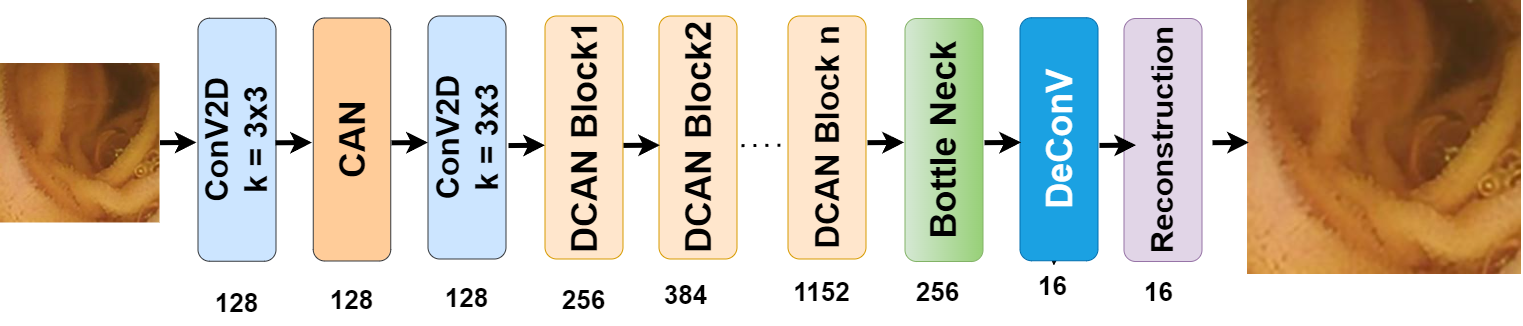
\includegraphics[width=0.99\textwidth]{1_fff.drawio.png} 
    \caption{The network architecture of proposed model \emph{DCAN}, where $k$ denotes kernel size and numerical values mentioned below every layer indicates size of output features.}
    \label{fig:label6.8}
\end{figure*}
The architecture of the proposed model for the task of SR of WCE images for upscaling factors $\times 4$ is depicted in Fig.~\ref{fig:label6.8}. It can be observed that the WCE LR image is given to a convolution layer first to learn low-level features. After this, a single CAN layer is added to learn the features channel wise from the LR image. Subsequently, a series of DCAN blocks are employed to learn high-level features. Towards the end, the bottleneck layer is used to decrease the input feature maps and finally, the deconvolution layer is employed to upsample the feature images, and the output of reconstruction layer generates an SR image.
%which is then provided as an input to CAN which extracts the features channel wise from the image and passes it to series of DCAN blocks to extract high-level features from LR images. 
%Figure ~\ref{fig:label6.8} depicts the architecture of the proposed method for the task of WCE image SR for upscaling factors $\times 4$. 
%The input WCE LR images applied to  a convolution layer to learn low-level features. After this, a single Channel Attention (CA) layer is added to learn the features channel wise from the image. Subsequently, a series of DCAN blocks are employed to learn high-level features. %As a result, each layer in the DCAN receives the input of feature maps from all preceding layers. 
%This design allows to enhance details and promotes feature reuse throughout the network, leading to more comprehensive and expressive representations at higher layers. %DCAN also incorporates short paths between each layer and all other layers, promoting the smooth flow of information and mitigating the vanishing-gradient problem. 
\begin{figure}[h!]
    \centering
    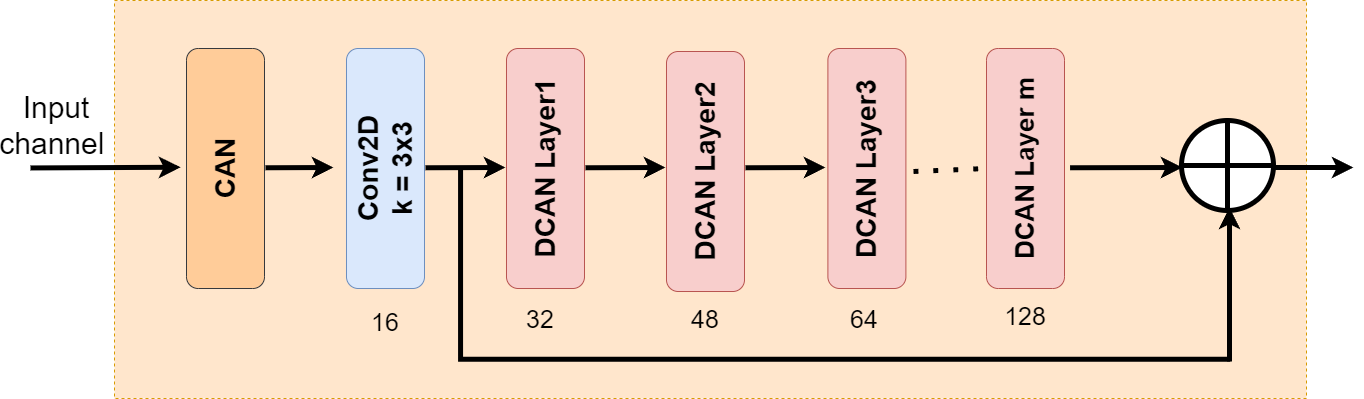
\includegraphics[width=0.5\textwidth]{2.drawio (4).png} %[totalheight=1.2in]
    \caption{The network architecture of DCAN block used in proposed model-\emph{DCAN}. The values below every layer indicate the number of output features.}
    \label{fig:label6.9}
\end{figure}
\subsection{DCAN Block}
In the proposed network, we utilize DCAN blocks as fundamental building unit. This design allows to enhance details and promotes feature reuse throughout the network, leading to more comprehensive and expressive representations at higher layers. The network architecture of DCAN block is depicted in Fig.~\ref{fig:label6.9}. There are $n$ number of DCAN blocks used in our architecture, which we fix to $8$ empirically. Each DCAN block consists Channel Attention Network (CAN), one convolution layer and $m$ number of DCAN layers (i.e., $m=8$) that enable to extract high-level features in the output image. Moreover, one skip connection is added to avoid vanishing-gradient problem. The block schematic DCAN layer is displayed in Fig.~\ref{fig:label6.10} (a). Each DCAN layer consists of a convolution layer having kernel size $3\times3$ and Relu activation function with short skip connection. Thus, the proposed model consists short skip connections and also global skip connections for effective learning and also to avoid gradient problem. 
%These DCAN layers are increasing number of features linearly by growth rate which is set to 16 and both the low level features and high level features are added using a short skip connection as shown in Fig.~\ref{fig:label6.10} (a). Further, each DCAN block consists of $m$ DCAN layers which we have taken as 8, generating a total of 16 * 8 feature maps, as each DCAN layer increases the output count of feature maps by 16. Hence the number of feature growth from each DCAN block is 128. Hence the number of features after 8 dense blocks gets to 1152.


\begin{figure}[h!]
    \centering
    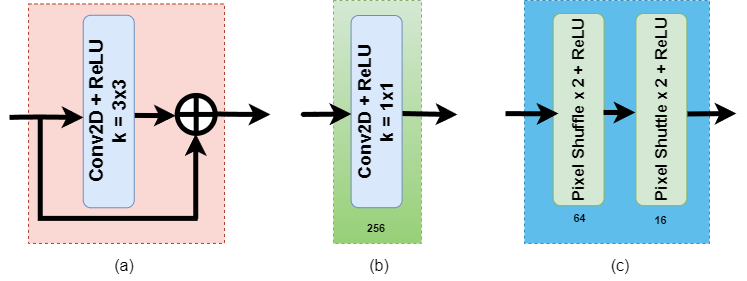
\includegraphics[width=0.5\textwidth]{fi.drawio (2).png} % [totalheight=1.2in]
    \caption{The design of (a) DCAN Layer, (b) Bottleneck Layer and (c) Deconvolution Layer in the proposed method.}
    \label{fig:label6.10}
\end{figure}

\subsection{Channel Attention Network (CAN)}
The earlier CNN-based SR methods \cite{SRCNN, VDSR, DRCN, ResNet, EDSR, SRDensenet}, treat LR channel-wise features equally, which is not optimal for real-world cases. To address this issue and focus the network on more informative features, CAN mechanism is proposed in RCAN \cite{RCAN} that exploits the interdependencies among feature channels. Generating different attention for each channel-wise feature is a crucial step in this mechanism. An LR information contains both low-frequency and high-frequency components that are valuable for SR. However, the low-frequency parts are relatively homogeneous, while the high-frequency components typically correspond to regions with edges, texture, and other details. Second, each filter in the convolution layer operates within a local receptive field, which limits its ability to exploit contextual information beyond the local region. Thus, the use of CA in the proposed method is helpful to learn the features effectively by assigning proper weights to each feature. The architecture for CAN is depicted in Fig.~\ref{fig:label6.11}. It consists of adaptive average pooling with a convolution layer having kernel size $3\times3$, attached with a ReLU activation function, which is passed to another convolution layer having kernel $1\times1$, and a skip connection is used to add the input values with the output of sigmoid function.
\begin{figure}[h!]
    \centering
    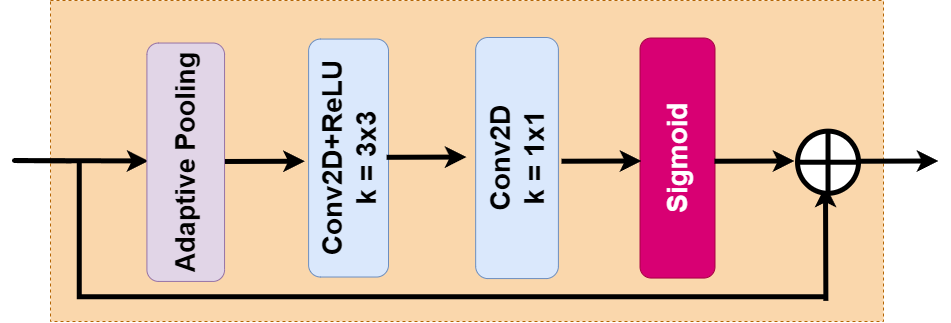
\includegraphics[width=0.5\textwidth]{4.drawio_fff.png} % [totalheight=1.2in]
    \caption{The architecture design of Channel Attention Network (CAN) used in \emph{DCAN} model.}
    \label{fig:label6.11}
\end{figure}


\subsection{BottleNeck Layer}
In order to enhance the compactness and computational efficiency of the model, we utilize a bottleneck layer to decrease the quantity of feature maps prior to their input into the deconvolution layers. The bottleneck layer shown in Fig.~\ref{fig:label6.10}(b) is used to reduce the output features from DCAN blocks to a lower dimension. It consists of a convolution layer having kernel size $1\times1$ with ReLU activation function. In our proposed model, we are reducing the features to 256 features using the bottleneck layer. 
%The bottleneck layer is used to reduce the number of parameters in the network, and also to speed up the training process. These layers then convert the feature maps from the LR space to the HR space. Hence we obtain 256 output features that are mapped from the 1152 features emitted by the stacked DCAN blocks.

\subsection{Deconvolution and Reconstruction Layers}
Deconvolution layers can be seen as the inverse operation of convolution layers, allowing for the learning of diverse upscaling kernels that work together to predict HR images. It provides two advantages: By conducting computations in the LR space, the SR reconstruction process is accelerated. %This approach significantly reduces the computational cost by a factor equal to the square of the upsampling factor employed. 
Additionally, the inclusion of deconvolution layer enables the utilization of contextual information from LR images to infer high-frequency details.
The network design of Deconvolution layer consists of two pixel-shuffle layers as shown in Fig.~\ref{fig:label6.10}(c), where each layer upsamples the image by a factor of $\times2$. Pixel-shuffle rearranges the feature maps by reshaping them into a higher resolution. It then rearranges the pixel values to get the final image. We are using two pixel-shuffle layers which give us total  upsampling of factor $4$. %As we are using 2 Pixel shufflers of factor 2, our output number of features will be divided by its squared value 4, hence the number of features after first pixel shuffler are 64 taking 256 feature maps as input from the bottleneck layer, while after the second pixel shuffler, we get 16 feature maps as output. This results in a better quality of the reconstructed image.
Finally, a reconstruction layer, consisting of a convolution layer with a $3\times3$ kernel, is used to generate SR images from the feature maps in the RGB space.
%The reconstruction layer is used to get the number of features that we have given in input image. 
%In our proposed method, we are using 3 feature maps for training on RGB channel and 1 feature map for training on the Y channel of the YCbCr color space.
%\begin{figure}[h!]
    %\centering
    %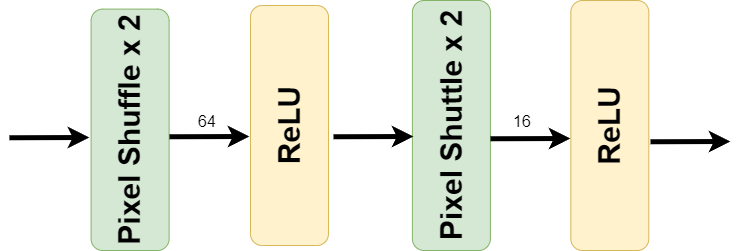
\includegraphics[totalheight=1.2in]{5_final.drawio.png}
   % \caption{Deconvolution Layer used for upscaling images in our DCAN model.}
   % \label{fig:label6.12}
%\end{figure}


\begin{figure*}[!t]
    % \centering
    % \includegraphics[totalheight=1.2in]{520_final_result.png}
    % \caption{Deconvolution Layer}
    % \label{fig:label6.12}
    % \centering
    % \begin{subfigure}
    %     \includegraphics{520/520_box.png}
    % \end{subfigure}
    % \hfill
    % \begin{subfigure}[b]{0.3\textwidth}
    %     \centering
    %     \includegraphics{520/520_bicubic.jpg}
    %     \caption{Bicubical}
    %     \vfill
    %     \includegraphics{520/520_Bicubical_ssim.jpg}
    %     \caption{Bicubical kernel}
    % \end{subfigure}
    \minipage{0.24\textwidth}
        \centering
        \includegraphics[width=\linewidth]{Figures/520/520_box.png}
    
    \endminipage\hfill
    \minipage{0.12\textwidth}
        \centering
        \includegraphics[width=\linewidth]{Figures/520/520_bicubic.jpg}
        
        \vfill
        \includegraphics[width=\linewidth]{Figures/520/520_Bicubical_ssim.jpg}
         
    \endminipage\hfill
    \minipage{0.12\textwidth}
        \centering
        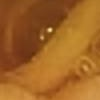
\includegraphics[width=\linewidth]{Figures/520/520_SRGAN.jpg}
        
        \vfill
        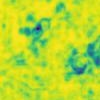
\includegraphics[width=\linewidth]{Figures/520/520_SRGAN_ssim.jpg}
        
    \endminipage\hfill
    \minipage{0.12\textwidth}
        \centering
        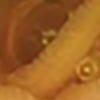
\includegraphics[width=\linewidth]{Figures/520/520_cycleGAN.jpg}
        
        \vfill
        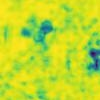
\includegraphics[width=\linewidth]{Figures/520/520_cycleGAN_ssim.jpg}
        
    \endminipage\hfill
    \minipage{0.12\textwidth}
        \centering
        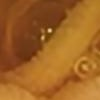
\includegraphics[width=\linewidth]{Figures/520/520_Densenet.jpg}
        
        \vfill
        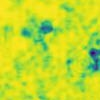
\includegraphics[width=\linewidth]{Figures/520/520_DenseNet__ssim.jpg}
        
    \endminipage\hfill
    \minipage{0.12\textwidth}
        \centering
        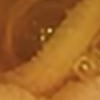
\includegraphics[width=\linewidth]{Figures/520/520_RCAN.jpg}
       
        \vfill
        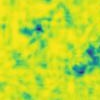
\includegraphics[width=\linewidth]{Figures/520/520_RCAN_ssim.jpg}
        
    \endminipage\hfill
    \minipage{0.12\textwidth}
        \centering
        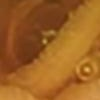
\includegraphics[width=\linewidth]{Figures/520/520_proposed.jpg}
        
        \vfill
        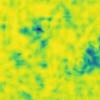
\includegraphics[width=\linewidth]{Figures/520/520_proposed_ssim.jpg}
        
    \endminipage\hfill
    %\caption{Patch analysis of images on different models using perceptual technique and attention maps }

\minipage{0.24\textwidth}
        \centering
        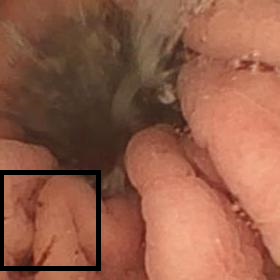
\includegraphics[width=\linewidth]{Figures/906/906_border.png}
        
    \endminipage\hfill
    \minipage{0.12\textwidth}
        \centering
        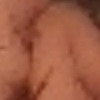
\includegraphics[width=\linewidth]{Figures/906/906_Bicubical.jpg}
        
        \vfill
        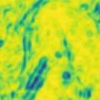
\includegraphics[width=\linewidth]{Figures/906/906_Bicubical_ssim.jpg}
        
    \endminipage\hfill
    \minipage{0.12\textwidth}
        \centering
        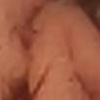
\includegraphics[width=\linewidth]{Figures/906/906_SRGAN.jpg}
        
        \vfill
        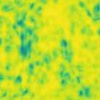
\includegraphics[width=\linewidth]{Figures/906/906_SRGAN_ssim.jpg}
        
    \endminipage\hfill
    \minipage{0.12\textwidth}
        \centering
        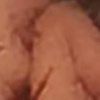
\includegraphics[width=\linewidth]{Figures/906/906_cycleGAN.jpg}
        
        \vfill
        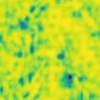
\includegraphics[width=\linewidth]{Figures/906/906_cycleGAN_ssim.jpg}
        
    \endminipage\hfill
    \minipage{0.12\textwidth}
        \centering
        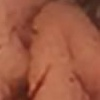
\includegraphics[width=\linewidth]{Figures/906/906_Densenet.jpg}
        
        \vfill
        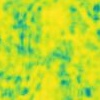
\includegraphics[width=\linewidth]{Figures/906/906_densenet_ssim.jpg}
        
    \endminipage\hfill
    \minipage{0.12\textwidth}
        \centering
        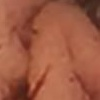
\includegraphics[width=\linewidth]{Figures/906/906_RCAN.jpg}
        
        \vfill
        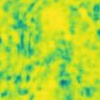
\includegraphics[width=\linewidth]{Figures/906/906_RCAN_ssim.jpg}
        
    \endminipage\hfill
    \minipage{0.12\textwidth}
        \centering
        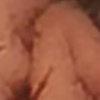
\includegraphics[width=\linewidth]{Figures/906/906_proposed.jpg}
        
        \vfill
        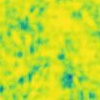
\includegraphics[width=\linewidth]{Figures/906/906_proposed_ssim.jpg}
        
    \endminipage\hfill
   % \caption{Patch analysis of images on different models using perceptual technique and attention maps }

\minipage{0.24\textwidth}
        \centering
        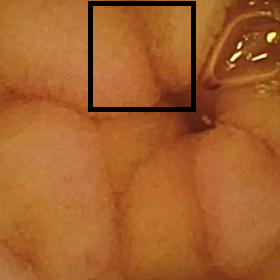
\includegraphics[width=\linewidth]{Figures/983/983_box.png}
        HR
    \endminipage\hfill
    \minipage{0.12\textwidth}
        \centering
        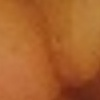
\includegraphics[width=\linewidth]{Figures/983/983_Bicubical.jpg}
         \\
        \vfill
        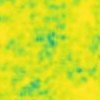
\includegraphics[width=\linewidth]{Figures/983/983_Bicubic__ssim.jpg}
        Bicubic \\
    \endminipage\hfill
    \minipage{0.12\textwidth}
        \centering
        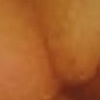
\includegraphics[width=\linewidth]{Figures/983/983_SRGAN.jpg}
         \\
        \vfill
        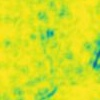
\includegraphics[width=\linewidth]{Figures/983/983_SRGAN__ssim.jpg}
        SRGAN \\
    \endminipage\hfill
    \minipage{0.12\textwidth}
        \centering
        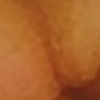
\includegraphics[width=\linewidth]{Figures/983/983_cycleGAN.jpg}
         \\
        \vfill
        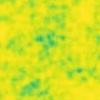
\includegraphics[width=\linewidth]{Figures/983/983_cycleGAN_ssim.jpg}
        CycleGAN \\
    \endminipage\hfill
    \minipage{0.12\textwidth}
        \centering
        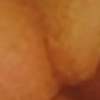
\includegraphics[width=\linewidth]{Figures/983/983_DenseNet.jpg}
         \\
        \vfill
        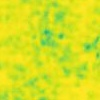
\includegraphics[width=\linewidth]{Figures/983/983_densenet_ssim.jpg}
        DenseNet\\
    \endminipage\hfill
    \minipage{0.12\textwidth}
        \centering
        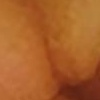
\includegraphics[width=\linewidth]{Figures/983/983_RCAN.jpg}
        \\
        \vfill
        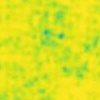
\includegraphics[width=\linewidth]{Figures/983/983_RCAN_ssim.jpg}
        RCAN\\
    \endminipage\hfill
    \minipage{0.12\textwidth}
        \centering
        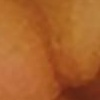
\includegraphics[width=\linewidth]{Figures/983/983_proposed.jpg}
      
        \vfill
        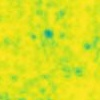
\includegraphics[width=\linewidth]{Figures/983/983_proposed_ssim.jpg}
        Proposed
    \endminipage\hfill
    \caption{Qualitative comparision of proposed models with state-of-the-art models using SSIM maps (where yellow region shows similarity and blue region shows disimilarity.)}
    \label{fig:qualanal}
\end{figure*}

\section{Experimental Analysis}
The design of the proposed model is validated by conducting subjective and quantitative evaluations. We empirically verify DCAN’s effectiveness %on a chosen dataset of 1000 images and compare% 
with state-of-the art architectures qualitatively by taking a patch from the output images from all state-of-the-art models. In addition, the same is verified quantitavively using different standard SR metrics such as Peak Signal to Noise Ratio (PSNR) \& Structural Similarity Index Metric (SSIM) and using perceptual metric i.e., Learned Perceptual Image Patch Similarity (LPIPS).  Finally, the statistical analysis of the proposed model are also presented in \emph{Supplementary material} due to space constraints. Our method is benchmarked against state-of-the-art models such as SRGAN \cite{SRGAN}, CycleGAN \cite{CycleGAN}, DenseNet \cite{SRDensenet}, and RCAN \cite{RCAN} for comparison purposes.  
\subsection{Dataset}
One of the novel contributions of the work is the creation of new derivative dataset from the available Kvasir Capsule Endoscopy Dataset \cite{data} consisting of WCE images.  
%The dataset consists of a segment of Kvasir-Capsule, a video capsule endoscopy dataset. 
In original Kvasir dataset, each image is in RGB color space with size of $336\times336$ pixels. The dataset contains a total of $47,236$ images, which are categorized according to different medical anomalies. As the original dataset contained redundant images with many border areas with black pixels, we have curated the dataset for the SR task by manually selecting images and removing redundant images from the Kavasir dataset.  %We used our prepared SR dataset for training and testing of proposed model.
%The proposed model used a portion of this dataset to evaluate the performance of the proposed method.
%\begin{table}[h!]
%\centering
%\caption{Table of original data set.}
%\begin{tabular}{ |c|c| }
%\hline
% Normal clean mucosa & 34338 \\
% Ileocecal valve & 4189 \\
% Reduced mucosal view & 2096 \\
% Pylorus    &    1529 \\
% Angiectasia         &     866 \\
% ulcer               &     854 \\
% Foreign body        &     766\\    
% Lymphangiectasia    &     592 \\
% Erosion             &     506 \\
% Blood - fresh       &     446 \\
 %Erythema            &      159 \\
 %Polyp               &      55 \\
% Blood - hematin     &       12 \\
 %ampulla of water    &        10 \\
%\hline
%\end{tabular}
%\label{Table:4.1}
%\end{table}
%\newline
The new SR dataset therefore consists of $10,000$ training images, $550$ validation images and $1000$ testing images \footnote{The dataset will be made available for researchers provide they have license agreement for original Kvasir Capsule dataset.}. As mentioned earlier, the WCE images from the original Kvasir dataset containing non-informative part in the border area. Those regions are removed manually through cropping resulting in images of $280\times280$ pixels for all images. The proposed model along with all other models are experimented on the new datset and SR results are generated.
%which was $336\times336$ pixels originally.
%As our original dataset images had redundancy, we used a subset of our original dataset consisting of 10,000 images. With that 1000 testing images were also taken from the original dataset, different from the training images. The corner of the images are complete black spaces in all the images of dataset that doesn't contain any information so we feed the network with cropped images, that didn't have any blank spot in the corners. After cropping, the resolution of the cropped images is $280 \times 280$ pixels, which was $336 \times 336$ pixels originally. In order to accomplish the comparision of HR and SR images, we firstly use bicubic interpolation method to downsample the size of HR image by a factor of 4 and make LR-HR pair of all the training images. The final training of all the models was done on this dataset. Hence we used 10,000 images of size $70 \times 70$ as our LR training images and obtained $280 \times 280$ pixels image as our output.

\subsection{Training details}
Firstly, to prepare LR-HR pair of WCE images, we consider the original images as the HR image and applied bicubic down-sampling with factor $\times 4$ and obtained LR image. These LR-HR pairs are fed to the proposed model to train it to generate SR images. Further, each LR image has also been transformed into $YCbCr$ space and only the $Y$-channel was used for training which represents a gamma-encoded channel that predominantly contains high-level feature information. On the other hand, the Cb and Cr channels are chroma-encoded channels that do not contain as many high-level features %\kr{This detail should also come in proposed approach. Right now, I am a bit confused about the RGB Ycbcr part. The reviewer will also be confused.}.
To save computational time during the process and improve the extraction of high-level features in the SR image, the Cb and Cr channels are directly interpolated and added to the output image. The training process aimed to minimize the loss function, which was taken as the Mean Squared Loss (MSE). The training was carried out for a total of $300$ epochs with a batch size of $32$. Additionally, the Adam optimizer was used with a learning rate of $0.0001$. This protocol was used on all the state-of-the-art models and SR results are generated. While testing, we use YCbCr space of test LR image to generate SR image.

%we firstly use bicubic interpolation method to downsample the size of HR image by a factor of 4 and make LR-HR pair of all the training images.
%on a patch of the image, each of size 100x100, and on the Y channel of the YCbCr channel.  Meanwhile, the $Y$ channel is utilized for training the model.
%The DCAN is designed to improve image processing by focusing on important features and details.

\subsection{Comparison with state-of-the-art models}

\textit{Qualitative Analysis:}
The qualitative comparison of various SR methods on scaling factor of $\times4$ is depicted in Fig.~\ref{fig:qualanal}. One can inspect by looking at the zoomed-in patches that the proposed model generates better SR solutions than other models. %\kr{the results are not very convincing. Is there any better way to visualize this? Different color space?. Kishor- tried with heat map but giving same results..}.
%For Qualitative (Visual) comparision of our proposed model with the state-of-the-art models, we have taken a patch of $100 \times 100$ pixels from the HR image of $280 \times 280$ and compared that patch taken from the output testing images from all SOTA models and our proposed model. 
Also, the SSIM map of each patch is shown below the patch SR image, which shows the similarity between generated SR and HR images. The yellow part in SSIM maps shows the similarity between SR and HR images. However, the green and blue regions in SSIM maps show the dissimilarity between SR and HR images. We can observe that the proposed model has more similar parts than the other methods.  In the first row SSIM maps in Fig.~\ref{fig:qualanal}, it can be observed that the bicubic output image exhibits the highest dissimilarity. Comparatively, other models such as RCAN and DenseNet perform better than other models as well as the bicubic method. However, the proposed model demonstrates the lowest dissimilarity among the bicubic method and all other state-of-the-art models. Additionally, in second row, it is apparent that SRGAN and DenseNet exhibit better performance in comparison. However, the proposed model demonstrates the highest structural similarity, indicating superior performance in terms of preserving the structural characteristics of the image. 
%more similar and the GREEn and blue part shows the dissimilarity SSIM maps tells us the similarity between two images by marking that region yellow and marking the dissimilarity by marking blue region.
%Also, as the dissimilarity between the images is not easily visible, we are using SSIM maps, which tells us the index of image similarity between two images. As we can observe in Fig. \ref{fig:qualanal}, we have displayed all the SSIM maps which were generated by comparing patches of HR image with the output images from all the models, which are shown below the patches of output images. 
%As the name suggests SSIM maps tells us the similarity between two images by marking that region yellow and marking the dissimilarity by marking blue region. As the dissimilarity index increases the blue region gets more intense and dark. We can depict from the image that the dissimilarity is highest in the bicubic image while its the lowest in output image of our proposed model.
\subsubsection*{Quantitative Analysis}
To validate the SR results quantitatively, the average SSIM and PSNR values for the testing images of each model are provided in Table~\ref{quantal}. We calculated the average PSNR and SSIM on $Y$ channel as well as the RGB channels. From the table, it can be observed that the proposed DCAN model has the highest PSNR in both the Y channel and RGB channel, %indicating better peak signal-to-noise ratio compared to other models. 
Additionally, the DCAN model also demonstrates the highest SSIM values, implying better structural similarity. When considering LPIPS for perceptual image comparison, lower LPIPS values emphasize the model's ability to capture perceptual similarity effectively. Remarkably, the DCAN model exhibits the lowest LPIPS values among all the different models, suggesting superior perceptual similarity. 

\begin{table}[h!]
\centering
\caption{Quantitative comparison of the proposed model over other models using different metrics such as PSNR, SSIM and LPIPS on RGB and Y-channels.}% \kr{Is it possible to generate violing/box plots to show the mean and std-deviation?}}
\label{quantal}
\resizebox{0.49\textwidth}{!}{
\begin{tabular}{|l|cc|cc|c|}
\hline
Model & \multicolumn{2}{c|}{PSNR $\uparrow$}                                            & \multicolumn{2}{c|}{SSIM $\uparrow$}                                       & \multicolumn{1}{l|}{LPIPS$\downarrow$} \\ \cline{2-6} 
                       & \multicolumn{1}{c|}{Y-channel}        & \multicolumn{1}{c|}{RGB}     & \multicolumn{1}{c|}{Y-channel}       & \multicolumn{1}{c|}{RGB} & \multicolumn{1}{c|}{RGB}   \\ \hline
Bicubic                & \multicolumn{1}{c|}{38.1069}          & \multicolumn{1}{l|}{37.2111} & \multicolumn{1}{c|}{0.9296}          & 0.9057                   & 0.2310                     \\ \hline
SRGAN \cite{SRGAN}         & \multicolumn{1}{c|}{38.0377}          & 37.0021                      & \multicolumn{1}{c|}{0.9291}          & 0.9049                   & 0.1972                     \\ \hline
CycleGAN \cite{CycleGAN}      & \multicolumn{1}{c|}{38.0121}          & 36.9441                      & \multicolumn{1}{c|}{0.9123}          & 0.9012                   & 0.1984                     \\ \hline
DenseNet \cite{SRDensenet}   & \multicolumn{1}{c|}{39.6842}          & 38.8596                      & \multicolumn{1}{c|}{0.9401}          & 0.9369                   & 0.1353                     \\ \hline
RCAN \cite{RCAN}          & \multicolumn{1}{c|}{40.1438}          & 39.4613                      & \multicolumn{1}{c|}{0.9427}          & 0.9371                   & 0.1359                     \\ \hline
Proposed  & \multicolumn{1}{c|}{\textbf{40.2261}} & \textbf{39.5389}             & \multicolumn{1}{c|}{\textbf{0.9486}} & \textbf{0.9378}          & \textbf{0.1346}            \\ \hline
\end{tabular}
}
\end{table}
%\begin{table*}[h!]
%    \centering
%    \caption{PSNR, SSIM and LPIPS of all models.}
%    \resizebox{0.9\textwidth}{!}{%
%    \begin{tabular}{|c c c c|}
%  \hline
% 
%   \begin{tabular}{|c|}
%        Model \\
%        \hline
%%          \\
 %       Proposed \\
 %       \hline
 %       Bicubic \\
 %       \hline
 %       SRGAN \cite{SRGAN}\\
 %       \hline
 %       CycleGAN \cite{CycleGAN}\\
 %       \hline
 %       DenseNET \cite{SRDensenet} \\
 %       \hline
 %       RCAN\cite{RCAN}\\
 %       \hline
 %       \end{tabular}    
 %       & \begin{tabular}{|c|c|}
 %       \multicolumn{2}{|c|}{PSNR $\uparrow$}\\
 %       \hline
 %       Y-Channel & RGB \\
 %       \hline
 %       \textbf{40.2261} $\uparrow$ & \textbf{39.5389} $\uparrow$ \\
 %       \hline
 %       38.1069 & 37.2111 \\
 %       \hline
 %       38.0377 & 37.0021 \\
 %       \hline
 %       38.0121 & 36.9441 \\
 %       \hline
 %       39.6842 & 38.8596 \\
 %       \hline
 %       40.1438 & 39.4613\\
 %       \hline
 %       \end{tabular}  & \begin{tabular}{|c|c|}
 %       \multicolumn{2}{|c|}{SSIM $\uparrow$}\\
 %       \hline
 %       Y-Channel & RGB \\
 %       \hline
 %       \textbf{0.9486} $\uparrow$ & \textbf{0.9378} $\uparrow$ \\
 %       \hline
 %       0.9296 & 0.9057 \\
 %       \hline
 %       0.9291 & 0.9049 \\
 %       \hline
 %       0.9123 & 0.9012 \\
 %       \hline
 %       0.9401 & 0.9369 \\
 %       \hline
 %       0.9427 & 0.9371\\
 %       \hline
 %       \end{tabular}  & \begin{tabular}{|c|}
 %       LPIPS $\downarrow$\\
 %       \hline
%        RGB \\
%        \hline
%        \textbf{0.1346} $\downarrow$\\
%        \hline
%        0.2310\\
%        \hline
%        0.1972\\
%        \hline
%         0.1984\\
%         \hline
%        0.1353 \\
%        \hline
%        0.1359 \\
%        \hline
%        \end{tabular} \\
%    \hline
%\end{tabular}%
%}
%\label{Table:6.1}
%\end{table*}
\subsubsection*{Statistical Analysis}
Finally, the statistical analysis is also conducted on the SR results of the proposed model along with the others to ensure the model consistency compared to state-of-the-art models. Standard deviation demonstrates the deviation in the values from the mean and hence it should be low for an algorithm. The values of standard deviation of each model are presented in Table~\ref{table:stanal}. As we can observe the values of our proposed model DCAN is lowest in comparision to all state-of-the-art models. From the given values, it can be noticed that while comparing PSNR consistency $Y$ channel has lower consistency than RGB channels and while comparing SSIM, its vice-a-versa. Thus, one can conclude from this that there is high peaks in $Y$-channel i.e., $Y$-channel works great on majority images and provides better PSNR values, but as it focuses only on $Y$-channel, the features in $Cb$ and $Cr$ channels are not percieved properly, so when the high-level features are in $Cb$ and $Cr$ channels, it loses important information which is although a rare case as all important information is in $Y$-channel majorly. The box-plot representations of the same is discussed in \emph{Supplementary material} due to space constraints. 
% Hence, RGB channel provides better consistency in peak signal to noise as compared to Y-channel 
%\as{I removed the sentence which is contradicting}
%\kr{This statement is contradicting.}. 


\begin{table}[]
\centering
\caption{The statistical comparison of the proposed model with other different methods using parameter of Standard Deviation of PSNR and SSIM values over mean values in RGB and Y-channels.}
\label{table:stanal}
\begin{tabular}{|l|cc|cc|c|}
\hline
Model & \multicolumn{2}{c|}{STD. dev. of PSNR $\downarrow$}                                            & \multicolumn{2}{c|}{STD. dev. of SSIM $\downarrow$}            \\ \cline{2-5} 
                       & \multicolumn{1}{c|}{Y-channel}        & \multicolumn{1}{c|}{RGB}     & \multicolumn{1}{c|}{Y-channel}       & \multicolumn{1}{c|}{RGB} \\ \hline
Bicubic                & \multicolumn{1}{c|}{3.8943}          & \multicolumn{1}{l|}{2.2102} & \multicolumn{1}{c|}{0.0353}          & 0.0347                  \\ \hline
SRGAN \cite{SRGAN}                 & \multicolumn{1}{c|}{3.3490}          & 2.6924                     & \multicolumn{1}{c|}{0.0348}          & 0.0324                                    \\ \hline
CycleGAN \cite{CycleGAN}              & \multicolumn{1}{c|}{3.6802}          & 2.1937                     & \multicolumn{1}{c|}{0.0356}          & 0.0319                                     \\ \hline
DenseNet \cite{SRDensenet}             & \multicolumn{1}{c|}{4.2025}          & 3.1996                      & \multicolumn{1}{c|}{0.0378}          & 0.0372                                    \\ \hline
RCAN  \cite{RCAN}                 & \multicolumn{1}{c|}{3.5612}          & 2.8753                      & \multicolumn{1}{c|}{0.0367}          & 0.0350                                \\ \hline
Proposed               & \multicolumn{1}{c|}{\textbf{3.0006}} & \textbf{2.0186}             & \multicolumn{1}{c|}{\textbf{0.0270}} & \textbf{0.0306}                    \\ \hline
\end{tabular}
\end{table}



\section{Conclusion}
%In this paper, we address the super-resolution of WCE images. 
Due to the hardware limitations of the WCE sensors, the captured data results in coarser resolution which affects the diagnosis accuracy of the diseases. We present a new SR approach \emph{DCAN} using dense connections and channel attention modules to convert LR images to SR images. As the proposed network integrates the advantages of Channel Attention Network (CAN) from RCAN and utilizes short dense connections inspired by DenseNet, the proposed approach is able to effectively extract details from LR observations.
% A new dataset consisting of $10,000$ samples has been created for this task and accuracy of the proposed method is justified by comparing it with various other state-of-the-art methods. 
Experiments show that the proposed  network can perform better than other  existing state-of-the-art SR models both quantitatively and qualitatively. The results are supported with a detailed analysis of quality assessment metrics such as PSNR, SSIM and LPIPS and statistical analysis of obatained results. A future direction in this work is to focus on improving the perceptual quality and assess it with medical practitioners. 

%we have shown evaluation of several state-of-the-art models for the task of Image Super Resolution in wireless capsule endoscopy images and conducted a series of experiments with different model architectures, including SRGAN, CycleGAN, Densenet  and RCAN. Based on the insights gained from these experiments, we proposed our noble network, DenseNET with Channel Attention Network (DCAN) architecture, which outperformed all existing SOTA models, not only in terms of achieving the best values for all the image quality assessment metrics such as PSNR,SSIM and LPIPS, but also in terms of consistency, as measured by statistical parameters such as standard deviation and box plots.




%\clearpage

%\begin{thebibliography}{00}
%%\bibitem{WCE} Prabhananthakumar Muruganantham, Senthil Murugan Balakrishnan, A survey on deep learning models for wireless capsule endoscopy image analysis, International Journal of Cognitive Computing in Engineering, Volume 2, 2021, Pages 83-92, ISSN 2666-3074.
%%\bibitem{WCE2} Sushma B., Aparna P., Recent developments in wireless capsule endoscopy imaging: Compression and summarization techniques, Computers in Biology and Medicine, Volume 149, 2022, 106087, ISSN 0010-4825.
%%\bibitem{WCE3}Gilja OH, Hatlebakk JG, Odegaard S, Berstad A, Viola I, Giertsen C, Hausken T, Gregersen H. Advanced imaging and visualization in gastrointestinal disorders. World J Gastroenterol. doi: 10.3748/wjg.v13.i9.1408. PMID: 17457973; PMCID: PMC4146926.
%%\bibitem{6}C. F. Sabottke and B. M. Spieler, “The effect of image resolution on deep learning in radiography,” Radiology:Artificial Intelligence, vol. 2, no. 1, p. e190015, 2020.
%%\bibitem{SISR}Honggang Chen, Xiaohai He, Chao Ren, Linbo Qing, Qizhi Teng, CISRDCNN: Super-resolution of compressed images using deep convolutional neural networks, Neurocomputing, Volume 285,2018, Pages 204-219, ISSN 0925-2312.
%%\bibitem{diffal-endo} D. Huang and H. Liu, “A short survey of image super resolution algorithms,” Journal of Computer Science Technology Updates, vol. 2,pp. 19–29, 2015.
%%\bibitem{SRCNN} C. Dong, C. C. Loy, and X. Tang, “Accelerating the super-resolution convolutional neural network,” in European conference on computer vision. Springer, 2016, pp. 391–407.
%%\bibitem{VDSR} Kim, J., Kwon Lee, J., Mu Lee, K.: Accurate image super-resolution using very deep convolutional networks. In: CVPR. (2016)
%%\bibitem{DRCN} Kim, J., Kwon Lee, J., Mu Lee, K.: Deeply-recursive convolutional network for
%image super-resolution. In: CVPR. (2016)
%\bibitem {ResNet} He, K., Zhang, X., Ren, S., Sun, J.: Deep residual learning for image recognition. In: CVPR. (2016)
%\bibitem{EDSR}Lim, B., Son, S., Kim, H., Nah, S., Lee, K.M.: Enhanced deep residual networks
%for single image super-resolution. In: CVPRW. (2017)
%\bibitem{SR Densenet} Tong Tong, Gen Li, Xiejie Liu, and Qinquan Gao. Image super-resolution using dense skip connection, 2017.
%\bibitem{RCAN} Yulun Zhang, Kunpeng Li, Kai Li, Lichen Wang, Bineng Zhong, and Yun Fu. Image super-resolution using very deep residual channel attention networks, 2018.
%\bibitem{perploss}Johnson, J., Alahi, A., Fei-Fei, L.: Perceptual losses for real-time style transfer and super-resolution. In: ECCV. (2016)
%\bibitem{perpsimi}Gatys, L., Ecker, A.S., Bethge, M.: Texture synthesis using convolutional neural
%networks. In: NIPS. (2015)
%\bibitem{perpsimi2}Bruna, J., Sprechmann, P., LeCun, Y.: Super-resolution with deep convolutional
%sufficient statistics. In: ICLR. (2015)
%\bibitem{contextloss} Mechrez, R., Talmi, I., Shama, F., Zelnik-Manor, L.: Maintaining natural image statistics with the contextual loss. arXiv preprint arXiv:1803.04626 (2018)
%\bibitem{SRGAN} Christian Ledig, Lucas Theis, Ferenc Huszar, Jose Caballero, Andrew Cunningham, Alejan-dro Acosta, Andrew Aitken, Alykhan Tejani, Johannes Totz, Zehan Wang, and Wenzhe Shi.
%Photo-realistic single image super-resolution using a generative adversarial network, 2016.
%\bibitem{MPDGAN} O. -Y. Lee, Y. -H. Shin and J. -O. Kim, "Multi-Perspective Discriminators-Based Generative Adversarial Network for Image Super Resolution," in IEEE Access, vol. 7, pp. 136496-136510, 2019.
%\bibitem{DMGAN} Minfeng Zhu and Pingbo Pan and Wei Chen and Yi Yang, DM-GAN: Dynamic Memory Generative Adversarial Networks for Text-to-Image Synthesis, 2019.
%\bibitem{CGAN} Mehdi Mirza and Simon Osindero, Conditional Generative Adversarial Nets, arXiv preprint arXiv: 1411.1784 (2018).
%\bibitem{LAPGAN} Emily Denton and Soumith Chintala and Arthur Szlam and Rob Fergus, Deep Generative Image Models using a Laplacian Pyramid of Adversarial Networks, 2015.
%\bibitem{CycleGAN} Jun-Yan Zhu, Taesung Park, Phillip Isola, Alexei A. Efros, Unpaired Image-To-Image Translation Using Cycle-Consistent Adversarial Networks, 2017.
%\bibitem{ESRGAN} Xintao Wang, Ke Yu, Shixiang Wu, Jinjin Gu, Yihao Liu, Chao Dong, Chen Change Loy, Yu Qiao, Xiaoou Tang on Enhanced SRGAN, Sept 2018.
%\bibitem{RaGAN} Jolicoeur-Martineau, A.: The relativistic discriminator: a key element missing from standard gan. arXiv preprint arXiv:1807.00734 (2018)
%\bibitem{Capsule} Prabhananthakumar Muruganantham and Senthil Murugan Balakrishnan on "A survey on deep learning models for wireless capsule endoscopy image analysis".
%\bibitem{data} Pia H. Smedsrud, Vajira Thambawita, Steven A. Hicks, Henrik Gjestang, Olsen Nedrejord, Espen Næss, Hanna Borgli, and Debesh Jha. Kvasir-capsule, a video capsule endoscopy dataset, 2021.
%\bibitem{DLSR} Zhihao Wang, Jian Chen, and Steven C. H. Hoi. Deep learning for image super-resolution: A survey, 2019.
%\bibitem{VDRCB} Lim, B., Son, S., Kim, H., Nah, S., Lee, K.M.: Enhanced deep residual networks
%for single image super-resolution, 2017.
%\bibitem{Adam} Diederik P. Kingma and Jimmy Ba. Adam: A method for stochastic optimization, 2014.
%\bibitem{GAN} Goodfellow, Ian J. and Pouget-Abadie, Jean and Mirza, Mehdi and Xu, Bing and Warde-Farley, David and Ozair, Sherjil and Courville, Aaron and Bengio, Yoshua. Generative Adversive Networks, June 2014.
%\bibitem{PSNR} Fernando A. Fardo and Victor H. Conforto and Francisco C. de Oliveira and Paulo S. Rodrigues, A Formal Evaluation of PSNR as Quality Measurement Parameter for Image Segmentation Algorithms, 1605.07116, 2016.
%\bibitem{SSIM} Zhou Wang and Bovik, A.C. and Sheikh, H.R. and Simoncelli, E.P. Image quality assessment: from error visibility to structural similarity, 2004.
%\bibitem{LPIPS} Zhang, Richard and Isola, Phillip and Efros, Alexei A. and Shechtman, Eli and Wang, Oliver, The Unreasonable Effectiveness of Deep Features as a Perceptual Metric, June 2018.

%\end{thebibliography}

%\include{mybibfile}
\balance
\bibliographystyle{ieeetr}
\bibliography{./IEEEabrv,mybibfile}
\end{document}